\documentclass[cn,blue,12pt]{elegantbook}
\input {d:/tex/preamble}

\excludecomment{note}
\excludecomment{solution}
\renewcommand \tkt[1]{{\CJKunderline[hidden=true, skip=true, thickness=1pt]{#1}}}

\begin{document}

\chapter{线段,角,相交线与平行线}%
\section{知识要点}%
\begin{comment}

\end{comment}
\label{cha:线段,角,相交线与平行线}
\begin{note}
  【对接教材】 人教: 七上第四章P125 -P141, 七下第五章Pl -P27,八上第十二章P48 -P52.P60 - P62; 北师: 七上第四章P106-P121,七下第二章P38-P54,八上第七章P161 -P177,八下第一章P15 -P16.P22 一 P35.\\
  【中考占比】10年3考,3分
\end{note}
\begin{zsyd}
\item 直线与线段
  \begin{zsyd}
  \item 两个基本事实
    \begin{zsyd}
    \item 直线的基本事实:\tkt{经过两点有且只有一条直线}(简记: \tkt{两点确定一条直线})

    \item 线段的基本事实:\tkt{两点之间的所有连线中线段最短}(简记:\tkt{两点之间线段最短})
    \end{zsyd}
  \item 线段的中点: 如图 \ding{172}, 点\(B\)把线段\(AC\)分成相等的两条线段\(AB\)与\(BC\),点B叫做线段AC的\tkt{中点},即有\tkt{\(AB=BC=\frac{1}{2}AC\)}\\
    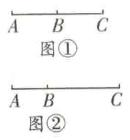
\includegraphics[width=0.15\linewidth]{20200519001.png}
  \item 线段的和与差: 如图 \ding{173},在线段\(AC\)上取一点\(B\),则有\(AB+\)\tkt{\(BC\)}\(=AC\); \(AB=\)\tkt{\(AC\)}\(-BC\); \(AC-AB=\)\tkt{\(BC\)}
  \end{zsyd}
\item 角及角平分线
  \begin{zsyd}
  \item 余角
    \begin{zsyd}
    \item 定义: 如果\tkt{两个角的和}等于\(90^\circ\).那么这两个角互为余角.
    \item 性质: 同角(等角)的余角\tkt{相等}
    \end{zsyd}
  \item 补角
    \begin{zsyd}
    \item 定义: 如果两个角的和等于\tkt{\(180 ^\circ\)},那么这两个角互为补角.
    \item 性质: 同角(等角)的补角\tkt{相等}
    \end{zsyd}
  \item 角平分线
    \begin{zsyd}
    \item 定义: 从一个角的\tkt{顶点}引出一条\tkt{射线},把这个角分成\tkt{两个完全相同的角},这条射线叫做这个角的角平分线.
    \item 性质:\tkt{角平分线上的点到角两边的距离相等}.
    \item 逆定理:角的内部到角两边\tkt{距离相等}的点在角的平分线上
    \end{zsyd}
  \end{zsyd}
\item 相交线
  \begin{zsyd}
  \item 角
    \begin{zsyd}
    \item 对顶角性质:对顶角 \tkt{相等}
    \item 邻补角性质:邻补角之和等于\tkt{\(180^\circ\)}
    \end{zsyd}
  \item 垂线性质
    \begin{zsyd}
    \item 在同一平面内, 过一点\tkt{有且只有一条}直线与已知直线垂
    \item 连接直线外一点与直线上各点的所有线段中,\tkt{垂线段}最短
    \item 点到直线的距离:\tkt{直线外一点到这条直线的垂线段的长度}
    \end{zsyd}
  \item 垂直平分线
    \begin{zsyd}
    \item 性质:\tkt{线段垂直平分线上的点到这条线段两个端点的距离相等}
    \item 判定:\tkt{到一条线段两个端点距离相等}的点,在这条线段的垂直平分线上
    \end{zsyd}
  \item 三线八角\\
    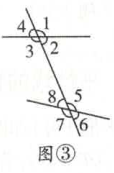
\includegraphics[width=0.15\linewidth]{20200519002.png}
    \begin{zsyd}
    \item 同位角:\(\angle 1\)与\tkt{\(\angle 5\)}, \(\angle 2\)与\tkt{\(\angle 6\)},\(\angle 3\)与\tkt{\(\angle 7\)},\(\angle 4\)与\tkt{\(\angle 8\)}
    \item 内错角:\(\angle 2\)与\tkt{\(\angle 8\)},\(\angle 3\)与\tkt{\(\angle 5\)}
    \item 同旁内角:\(\angle 3\)与\tkt{\(\angle 8\)},\(\angle 2\)与\tkt{\(\angle 5\)}
    \end{zsyd}
  \end{zsyd}
\item 平行线
  \begin{zsyd}
  \item 两个基本事实
    \begin{zsyd}
    \item 公理:经过直线外一点,\tkt{有且只有一条}直线与这条直线平行
    \item 推论:如果两条直线都与第三条直线平行,那么这两条直线也互相平行, 即如果 \(b // a,c // a\),那么\tkt{\(b // c\)}
    \item 注:在同一平面内, \tkt{垂直同一直线}的两条直线平行
    \end{zsyd}
  \item 平行线的性质与判定\\
    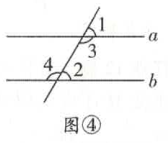
\includegraphics[width=0.15\linewidth]{20200519003.png}
    \begin{zsyd}
    \item \tkt{同位角相等}\(\iff\)两直线平行:
    \item \tkt{内错角相等}\(\iff\)判定 两直线平行:
    \item \tkt{同旁内角互补}\(\iff\)两直线平行:
    \end{zsyd}
  \end{zsyd}
\item 命题
  \begin{zsyd}
  \item 命题:判断一件事情的语句
  \item 真命题:\tkt{如果题设成立,那么结论一定成立},这样的命题叫做真命题
  \item 假命题:\tkt{题设成立时,不能保证结论一定成立},这样的命题叫做假命题
  \item 互逆命题:在两个命题中, 如果\tkt{第一个命题的题设是另一个命题的结论},而\tkt{第一个命题的结论是另一个命题的题设},那么这两个命题叫做互逆命题
  \end{zsyd}
\item 常见逻辑词
  \begin{zsyd}
  \item 都有(是),恰好,总有
  \item 可以为(是),可能是
  \item 不可能为
  \item 只有,只能是
  \end{zsyd}
\end{zsyd}

\section{中考真题}%

\subsection{补角的计算}%
\begin{zhenti}[resume]
\item 一个角的度数为\(20 ^\circ \),则它的补角的度数为\tkt{160\(^\circ\)}.
\end{zhenti}

\subsection{平行线的性质与判定}%
\begin{zhenti}[resume]
\item (2013江西8题3分)如图,在\(\Delta ABC\)中,\(\angle A=90^\circ\),点 在D在\(AC\)边上,\(DE // BC\),若\(\angle 1 =155 ^\circ \),则\(\angle B\)的度数为\tkt{\(65^\circ\)}.\\
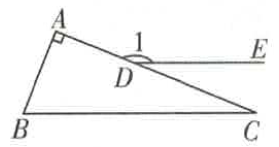
\includegraphics[width=0.2\linewidth]{20200602001.png}\\
\item (2010江西12题3分)一大门的栏杆如图所示,\(BA\)垂直于地面\(AE\)于点\(A\),\(CD\)平行于地面\(AE\),则\(\angle ABC + \angle BCD =\) \tkt{270}度.\\
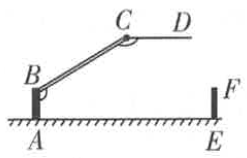
\includegraphics[width=0.2\linewidth]{20200602002.png}\\
\item (2019山西)如图,在\(\triangle ABC \)中\( AB=AC\),\(\angle A=30 ^\circ \),直线\(a // b\),顶点\(C\)在直线\(b\)上,直线\( a \)交\(AC\)于点\(E\),若\(\angle 1 = 145 ^\circ\),则\(\angle 2\)的度数是(\tkt{C})\\
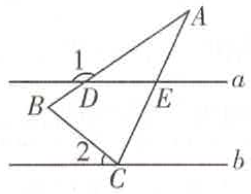
\includegraphics[width=0.2\linewidth]{20200602003.png}\\
  \begin{tasks}(4)
    \task \( 30^\circ \)
    \task \( 35^\circ\)
    \task \(40^\circ \)
    \task \( 45 ^\circ \)
  \end{tasks}
\item (2019济宁)如图,直线\(a,b\)被直线\(c\),\(d\)所截,若\(\angle 1 = \angle 2, \angle 3 = 125^\circ \),则\(\angle 4\)的度数是(\tkt{C})\\
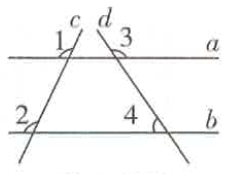
\includegraphics[width=0.2\linewidth]{20200602004.png}\\
  \begin{tasks}(4)
    \task \( 65^\circ \)
    \task \( 60^\circ \)
    \task \( 55^\circ \)
    \task \( 75 ^\circ \)
  \end{tasks}
\item (2019东营)将一副三角板(\(\angle A =30^\circ\),\( \angle E =45^\circ \))按如图所示方式摆放,使得\(BA // EF\),则\(\angle AOF\)等于(\tkt{A})\\
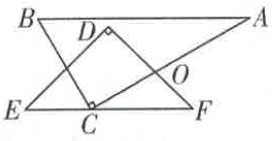
\includegraphics[width=0.2\linewidth]{20200602005.png}\\
  \begin{tasks}(4)
    \task \(75^\circ\)
    \task \(90^\circ\)
    \task \(105^\circ\)
    \task \(115^\circ\)
  \end{tasks}
\end{zhenti}

\subsection{核心素养}%
\begin{zhenti}[resume]
\item (2019毕节改编)如图,\(\Delta ABC\)中,\(CD\)是\(AB\)边上的高,\(CM\)是\(AB\)边上的中线,点\(C\)到边所在直线的距离是\tkt{线段CD的长度} .\\
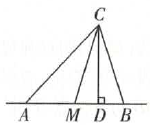
\includegraphics[width=0.2\linewidth]{20200602022.png}\\
\item \( \ding{172}\)是我们常用的折叠式小刀.图\( \ding{173}\)中刀柄外形是一个矩形挖去一个小半圆,其中刀片的两条边缘线可看成两条平行的线段,转动刀片时会形成图\( \ding{173}\)所示的\(\angle 1\)与\(\angle 2\),则\(\angle 1\)与\(\angle 2\)的度数和是\tkt{90}度\\
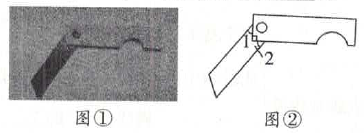
\includegraphics[width=0.6\linewidth]{20200602023.png}\\
\end{zhenti}

\section{强化训练}%

\subsection{逻辑词专项练习}%
\begin{enumerate}
\item 一个几何体的三视图形状都相同,大小均相等,那么这个几何体不可能是(\tkt{D})\\
\begin{tasks}(4)
\task 球\task 三棱锥\task 正方体\task 圆柱
\end{tasks}
\item 平面直角坐标系中,分别过点\(A(m,0)\),\(B(m+3,0)\)作垂直于\(x\)轴的直线\(l_1\)和\(l_2\),探究直线\(l_1,l_2\)与函数\(y = \frac{4}{x}\)的图象(双曲线)之间的关系,下列结论错误的是(\tkt{C})\\
\begin{tasks}(1)
\task 两条直线中总有一条与双曲线相交
\task 当\(m = 1\)时,两条直线与双曲线的交点到原点的距离相等
\task 当\(m<0\)时,两条直线与双曲线的交点都在\(y\)轴左侧
\task 当\(m>0\)时,两条直线与双曲线的交点都在\(y\)轴右侧
\end{tasks}
\item 如图,要得到\(AB//CD\),只需要添加一个条件,这个条件不可以是(\tkt{A})\\
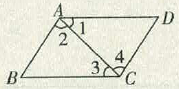
\includegraphics[width=0.2\linewidth]{20200602018.png}\\
\begin{tasks}(2)
\task \(\angle 1=\angle 3\)
\task \(\angle B+\angle BCD=180^\circ\)
\task \(\angle 2=\angle 4\)
\task \(\angle D+\angle BAD=180^\circ\)
\end{tasks}
\item 已知方程组\( \begin{cases} x+y=5\\ 2x-y=1\end{cases}\)的解恰好是\(\triangle ABC\)的两边长,则\(ABC\)的第三边的长不可能为(\tkt{D})\\
\begin{tasks}(4)
\task \(2\)
\task \(3\)
\task \(4\)
\task \(5\)
\end{tasks}
\item 如图,\(\angle MAN =60^\circ\),点\(B\)为\(AM\)上一点,以点\(A\)为圆心,任意长为半径画孤,交\(AM\)于点\(E\),交\(AN\)于点\(D\),再分别以点\(D\),\(E\)为圆心,大于\(\frac{1}{2}DE\)长为半径画弧,两弧交于点\(F\),作射线\(AF\),在\(AF\)上取点\(G\),连接\(BG\),过点\(G\)作\(GC\perp AN\),垂足为点\(C\),若\(AG=6\),则\(BG\)的长可以为(\tkt{D})\\
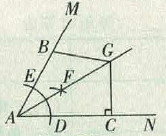
\includegraphics[width=0.2\linewidth]{20200602019.png}\\
\begin{tasks}(4)
\task \(1\)
\task \(2\)
\task \(\sqrt{3}\)
\task \(2\sqrt{3}\)
\end{tasks}
\item 若直线\(y = kx+k+1\)经过点\((m,n+3)\)和(\(m + 1\),\(2n-1\)),且\(0<k<2\),则\(n\)的值可以是(\tkt{D})\\
\begin{tasks}(4)
\task \(3\)
\task \(4\)
\task \(5\)
\task \(6\)
\end{tasks}
\begin{solution}
    代入两点坐标,得 \(k=n-4 \Rightarrow n=k+4 \Rightarrow 4<k<6\)
\end{solution}
\item 如图,已知\(\odot O\)的半径为\(5\),弦\(AB=8\),\(M\)是\(AB\)上任意一点,则线段\(OM\)的最小值只能是(\tkt{A})\\
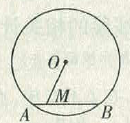
\includegraphics[width=0.2\linewidth]{20200602020.png}\\
\begin{tasks}(4)
\task \(3\)
\task \(4\)
\task \(4.5\)
\task \(5\)
\end{tasks}
\item 如图,在平面直角坐标系中,直线\(y= -\frac{1}{2}x+2\)分别交\(x\)轴、\(y\)轴于\(A,B\)两点,点\(P(1,m)\)在\( \triangle AOB\)内(包含边界),则\(m\)的值可能是(\tkt{A})\\
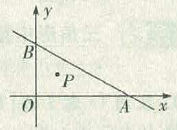
\includegraphics[width=0.2\linewidth]{20200602021.png}\\
\begin{tasks}(4)
\task \(1\)
\task \(2\)
\task \(3\)
\task \(4\)
\end{tasks}
\begin{solution}
    A,B,C代入求值.C选项注意不要用因式分解,因为不是求零点.
\end{solution}
\item 已知二次函数\(y=2mx^2 + (1 -m)x-1-m\),下面说法错误的是(\tkt{D})\\
  \begin{tasks}(1)
  \task 当\(m = 1\)时,函数图象的顶点坐标是\((0, -2)\)
  \task 当\(m = -1\)时,函数图象与\(x\)轴总有两个交点
  \task 函数图象必经过定点\((1,0),(-\frac{1}{2},-\frac{3}{2})\)
  \task 当\(m >0\)时,函数图象截\(x\)轴所得的线段长度都小于\(\frac{3}{2}\)
\end{tasks}
  \item 三角形有一条边是另一条边的\(2\)倍,并且有一个内角是\(30^\circ \),那么这个三角形(\tkt{D})\\
    \begin{tasks}(1)
\task 一定是直角三角形
\task 一定是钝角三角形
\task 不可能是直角三角形
\task 不可能是锐角三角形
\end{tasks}
\begin{solution}
    当另一条边为最大边时,直角三角形.当另一条边为次大边时,为钝角三角形.
\end{solution}
\item 关于\(x\)的一元二次方程\(ax^2+ bx -2 =0\)(\( a,b\)是常数,且\( a \ne 0\)),下列说法正确的是(\tkt{D})\\
    \begin{tasks}(1)
\task 若\(a =2\),则方程恰好有四个相等的实数根
\task 当\(b=0\)时,要使方程有实数根,\(a\)可以是\(-1\)
\task 若\(a<0\),则方程不可能有实数根
\task 若\(a>0\)则方程一定有两个不相等的实数根
\end{tasks}
\item 已知反比例函数\(y =\frac{2-k}{x}\)的图象在第一、三象限内,则\(k\)的值可以是\tkt{\(\tkt{-1}\)}.(写出满足条件的一个\(k\)的值即可)
\begin{solution}
        \(2-k>0\)即可
\end{solution}
\end{enumerate}
\subsection{综合题组1}%
(30分钟)
\begin{shiti}
\item 基础过关
  \begin{shiti}
  \item 与\(30 ^\circ\)的角互为余角的角的度数是(\tkt{B})\\
    \begin{tasks}(4)
      \task \(30 ^\circ\)
      \task \( 60^\circ \)
      \task \( 70^\circ \)
      \task \( 90 ^\circ \)
    \end{tasks}
  \item 如图,直线\(a,b\)被直线\(c\)所截,下列条件,不能判定直线\( a\)与\(b\)平行的是(\tkt{D})\\
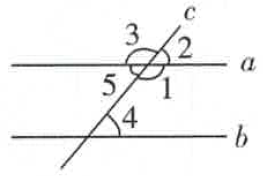
\includegraphics[width=0.2\linewidth]{20200602006.png}\\
    \begin{tasks}(4)
      \task \(\angle 2=\angle 4\)
      \task \(\angle 1+ \angle 4 =180^\circ\)
      \task \(\angle 5=\angle 4\)
      \task \(\angle 1=\angle 3\)
    \end{tasks}
  \item 如图,\(AB // CD\),\(\angle A =50^\circ \),则\(\angle 1\)的度数是(\tkt{C})\\
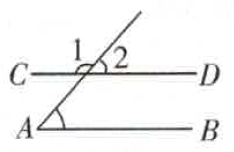
\includegraphics[width=0.2\linewidth]{20200602007.png}\\
    \begin{tasks}(4)
      \task \( 40^\circ \)
      \task \( 50 ^\circ  \)
      \task \( 130 ^\circ \)
      \task \( 150 ^\circ \)
    \end{tasks}
  \item 如图,直线\(AB // CD \),\(\angle C =36^\circ \),\( \angle E\)为直角,则\(\angle A\)等于(\tkt{C})\\
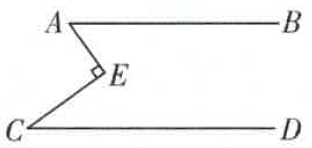
\includegraphics[width=0.2\linewidth]{20200602008.png}\\
    \begin{tasks}(4)
      \task \(36^\circ\)
      \task \(44^\circ\)
      \task \(54^\circ\)
      \task \(64^\circ\)
    \end{tasks}
\begin{solution}
        延长AE,得\(\angle C\)的余角等于\(\angle A\)
\end{solution}
  \item 如图,钟表上\(10\)点整时,时针与分针所成的角是(\tkt{B})\\
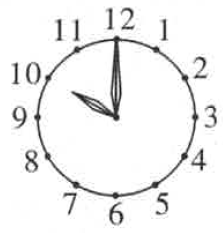
\includegraphics[width=0.2\linewidth]{20200602009.png}\\
    \begin{tasks}(4)
      \task \(30^\circ\)
      \task \(60^\circ\)
      \task \(90^\circ\)
      \task \(120^\circ\)
    \end{tasks}
\begin{solution}
        \(360 \times \frac{2}{12}=60^\circ\)
\end{solution}
  \item 将等腰直角三角形纸片和矩形纸片按如图方式叠放在一起,若\(\angle 1 =30 ^\circ \),则\(\angle 2\)的度数为(\tkt{B})\\
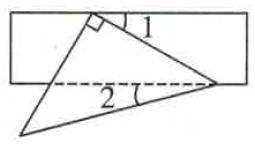
\includegraphics[width=0.2\linewidth]{20200602010.png}\\
    \begin{tasks}(4)
      \task \(10^\circ\)
      \task \(15^\circ\)
      \task \(20^\circ\)
      \task \(30^\circ\)
    \end{tasks}
\begin{solution}
        \(\angle 1\)的内错角加\(\angle 2 = 45^\circ\)\(\angle 2=45^\circ -\angle 1\)
\end{solution}
  \item 如图,在\(\triangle ABC \)中,\(\angle C=90^\circ\),\(AC =8, DC=\frac{1}{3}AD\),\(BD\)平分\(\angle ABC\),则点\(D\)到\(AB\)的距离等于(\tkt{C})\\
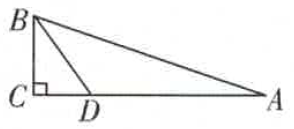
\includegraphics[width=0.2\linewidth]{20200602011.png}\\
    \begin{tasks}(4)
      \task \(4\)
      \task \(3\)
      \task \(2\)
      \task \(1\)
    \end{tasks}
\begin{solution}
角平分线到两边距离相等.所以\(D\)到\(AB\)的距离等于\(DC=2\)
\end{solution}
  \item 下列命题:\ding{172}直线外一点到这条直线的垂线段,叫做点到直线的距离;\ding{173}两点之间线段最短;\ding{174}相等的圆心角所对的弧相等;\ding{175}平分弦的直径垂直于弦.其中,真命题的个数是(\tkt{C})\\
    \begin{tasks}(4)
      \task \(1\)
      \task \(2\)
      \task \(3\)
      \task \(4\)
    \end{tasks}
\begin{solution}
        C.同圆或等圆,相等的圆心角所对的弧相等.
\end{solution}
  \item 如图,已知\( AB = 8 cm\),\(BD=3 cm\),\(C \)为\(AB\)的中点,则线段\(CD\)的长为\tkt{\(1\)}cm.\\
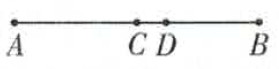
\includegraphics[width=0.2\linewidth]{20200602012.png}\\
  \item 我们学过用直尺和三角尺画平行线的方法,如图所示,直线\(a // b\)的根据是\tkt{同位角相等,两直线平行} .\\
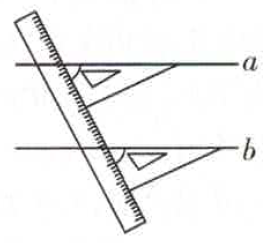
\includegraphics[width=0.2\linewidth]{20200602013.png}\\
  \item 如图,直线\(AB//CD\),直线\(EC\)分别与\(AB\),\(CD\)相交于点\(A\),点\(C\). \(AD\)平分\(\angle BAC\),已知\(\angle ACD =80 ^\circ \),则\(\angle DAC\)的度数为\tkt{\(50^\circ\)}.\\
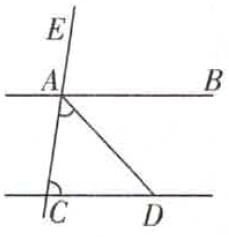
\includegraphics[width=0.2\linewidth]{20200602014.png}\\
  \item 如图,\(AB//CD\),\(AC//BD\),\(\angle 1 =28 ^\circ\),则\(\angle 2\)的度数为\tkt{\(28^\circ\)}.\\
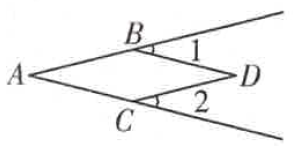
\includegraphics[width=0.2\linewidth]{20200602015.png}\\
  \end{shiti}
\item 满分冲关
  \begin{shiti}
  \item 将一副三角板按如图所示的位置摆放在直尺上,则\(\angle 1\)的度数为(\tkt{C})\\
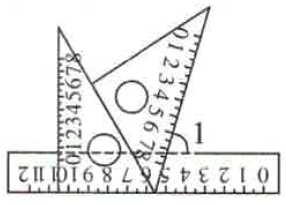
\includegraphics[width=0.2\linewidth]{20200602016.png}\\
    \begin{tasks}(4)
      \task \(60^\circ\)
      \task \(65^\circ\)
      \task \(75^\circ\)
      \task \(85^\circ\)
    \end{tasks}
\begin{solution}
        \(\angle 1\)的同位角等于\(180 - (65+45)=75^\circ\)
\end{solution}
  \item 如图,\(AD // CE\),\( \angle ABC = 100 ^\circ \),则\( \angle 2 - \angle 1\)的度数是\tkt{\(80^\circ\)}.\\
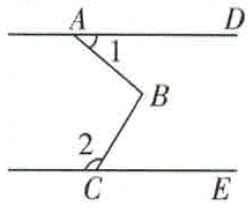
\includegraphics[width=0.2\linewidth]{20200602017.png}\\
\begin{solution}
    延长\(BC, \angle 2 + \angle D=180; \angle 1+\angle D=\angle ABC=80^\circ\),两式相减
\end{solution}
  \end{shiti}
\end{shiti}

\end{document}
